\documentclass[a4paper, 12pt]{article}

\newcommand{\languages}{french, english}

%%%%%%%%%%%%%%%%%%% Packages

%%%%% Tools

\usepackage{comment}
\usepackage{lipsum}
\usepackage{xstring}

%%%%% Document

\usepackage[pdfusetitle]{hyperref}

\usepackage{geometry}
\geometry{paper=a4paper,top=3.5cm,bottom=2.5cm,right=2.5cm,left=2.5cm}

\usepackage{fancyhdr}
\pagestyle{fancy}
\fancyhead[L]{}
\fancyhead[R]{\leftmark}
\fancyfoot[C]{\thepage}
\renewcommand{\headrulewidth}{0pt}

%%%%% Text

\usepackage[utf8]{inputenc}
\usepackage[T1]{fontenc}
\usepackage[parfill]{parskip}
\usepackage{csquotes}

\newlength{\mytextsize}
\makeatletter
\setlength{\mytextsize}{\f@size pt}
\makeatother

%%%%% Languages

\ifx\languages\undefined
	\usepackage[english, french]{babel}
\else
	\usepackage[\languages]{babel}
\fi

% english

\addto\captionsenglish{\def\figurename{Figure}}
\addto\captionsenglish{\def\tablename{Table}}

\newcommand{\st}{\text{s.t.}}

\IfStrEq{\languagename}{english}{
	\newcommand{\lgpreamble}{Preamble}
}

% french

\frenchbsetup{StandardLists=true}

\addto\captionsfrench{\def\figurename{Figure}}
\addto\captionsfrench{\def\tablename{Table}}
\addto\captionsfrench{\def\proofname{Preuve}}

\newcommand{\tq}{\text{t.q.}}
\newcommand{\cad}{c.-à-d. }
\newcommand{\Cad}{C.-à-d. }

\IfStrEq{\languagename}{french}{
	\newcommand{\lgpreamble}{Préambule}
}

%%%%% Styles

\usepackage[skip=\mytextsize]{caption}
\usepackage{float}
\usepackage{mdframed}
\usepackage{enumitem}
\usepackage{eurosym}
\usepackage{color}

\newcommand\caaption[1]{\caption{#1}\vspace{-1\mytextsize}}

%%%%% Mathematics

\usepackage{amsmath}
\usepackage{amssymb}
\usepackage{amsfonts}
\usepackage{bm}
\usepackage{esint}
\usepackage[makeroom]{cancel}

\newcommand{\fact}[1]{#1!}
\newcommand{\e}[1]{\mathbf{e}_{#1}}
\newcommand{\deriv}{\mathrm{d}}
\DeclareMathOperator{\tr}{tr}


%%%%% SI units

\usepackage[squaren,Gray,cdot]{SIunits}
\usepackage{sistyle}

\IfStrEq{\languagename}{french}{
	\SIdecimalsign{,}
}

%%%%% Chemistry

\usepackage[version=4]{mhchem}

%%%%% Table & Figure

\usepackage{array}
\usepackage{tabularx}
\usepackage{multirow}
\usepackage{multicol}
\newcolumntype{M}[1]{>{\centering\arraybackslash}m{#1}}
%\setlength\extrarowheight{0em}
\renewcommand{\arraystretch}{1.3}

\usepackage{wrapfig}
\usepackage{pgfplots}
\usepackage{tikz}
\usetikzlibrary{shapes.geometric, positioning}
\usepackage{graphics}
\usepackage{graphicx}
\pgfplotsset{axis on top, compat = 1.3}

%%%%%% Theorems and Definitions

\usepackage{amsthm}
\usepackage{thmtools}

\IfStrEq{\languagename}{english}{
	\newcommand{\lgthm}{Theorem}
	\newcommand{\lglem}{Lemma}
	\newcommand{\lgprop}{Proposition}
	\newcommand{\lgdefn}{Definition}
	\newcommand{\lghyp}{Hypothesis}
	\newcommand{\lgquest}{Question}
	\newcommand{\lgansw}{Answer}
	\newcommand{\lgexpl}{Example}
	\newcommand{\lgrmk}{Remark}
	\newcommand{\lgnote}{Note}
	\newcommand{\lgtip}{Tip}
}

\IfStrEq{\languagename}{french}{
	\newcommand{\lgthm}{Théorème}
	\newcommand{\lglem}{Lemme}
	\newcommand{\lgprop}{Proposition}
	\newcommand{\lgdefn}{Définition}
	\newcommand{\lghyp}{Hypothèse}
	\newcommand{\lgquest}{Question}
	\newcommand{\lgansw}{Réponse}
	\newcommand{\lgexpl}{Exemple}
	\newcommand{\lgrmk}{Remarque}
	\newcommand{\lgnote}{Note}
	\newcommand{\lgtip}{Conseil}
}

\theoremstyle{plain}
\newtheorem{thm}{\lgthm}[section]
\newtheorem{lem}{\lglem}[section]
\newtheorem{prop}{\lgprop}[section]

\theoremstyle{definition}
\newtheorem{defn}{\lgdefn}[section]
\newtheorem{hyp}{\lghyp}[section]
\newtheorem{quest}{\lgquest}[]

\declaretheorem[
name=\lgansw,
qed={\lower-0.3ex\hbox{$\triangle$}},
within=quest
]{answ}

\declaretheorem[
name=\lgexpl,
qed={\lower-0.3ex\hbox{$\triangle$}},
within=section
]{expl}

\theoremstyle{remark}
\newtheorem*{rmk}{\lgrmk}
\newtheorem*{note}{\lgnote}
\newtheorem*{tip}{\lgtip}

\begingroup
\makeatletter
\@for\theoremstyle:=definition,remark,plain\do{%
	\expandafter\g@addto@macro\csname th@\theoremstyle\endcsname{%
		\addtolength\thm@preskip\parskip
	}%
}
\endgroup

%%%% Others

\renewcommand{\qedsymbol}{$\blacksquare$}

\newcommand{\mytableofcontents}{
	\newpage
	\pagenumbering{roman}
	\tableofcontents
	\newpage
	\pagenumbering{arabic}
}

%%%%%%%%%%%%%%%%%%%

%%%%%%%%%%%%%%%%%%% Titlepage

\newcommand{\toptitle}{Dynamique des Systèmes \\[0.25em] Mécaniques}
\title{Project 1}
\newcommand{\subtitle}{One degree of freedom damped system}
\author{François \textsc{Rozet}}
\newcommand{\context}{University of Liège}
\date{\today}

%%%%%%%%%%%%%%%%%%% Others

\fancyhead[R]{\uppercase{D.S.M. -- Project 1}}

%%%%%%%%%%%%%%%%%%%

\begin{document}
	\newgeometry{margin = 2.5cm}
\makeatletter
\begin{titlepage}
	\begin{minipage}[t][0.425\textheight][t]{\textwidth}
		\begin{center}
			
\includegraphics[height=0.15\textheight]{include/resources/pdf/logo_uliege.pdf}
			\vfill
			\ifx\toptitle\undefined
				{\huge \textsc{Université de Liège}}
			\else
				{\huge \textsc{\toptitle}}
			\fi
			\vfill
		\end{center}
	\end{minipage}
	\vfill
	\begin{minipage}{\textwidth}
		\hspace{6pt}
		\begin{mdframed}[linewidth = 2pt, innertopmargin = 12pt, innerbottommargin = 12pt, leftline = false, rightline = false]
			\begin{center}
				{\huge \bfseries \@title}
			\end{center}
		\end{mdframed}
		\hspace{6pt}
	\end{minipage}
	\vfill
	\begin{minipage}[b][0.425\textheight][t]{\textwidth}
		\begin{center}
			\ifx\subtitle\undefined
			\else
				{\LARGE \subtitle}
			\fi
			\vfill
			{\large \@author}
			\vfill
			{\large \context \\[6pt] \@date}
		\end{center}
	\end{minipage}
\end{titlepage}
\makeatother
\restoregeometry

	{
		\begin{wrapfigure}{r}{0.35\textwidth}
			\centering
			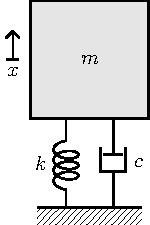
\includegraphics[width=0.3\textwidth]{resources/tikz/1dof_system/1dof_system.pdf}
			\caption{System}
		\end{wrapfigure}
		\part*{Setup}
		The system consists in a mass $m$ supported by a spring of stiffness $k$ and a viscous damper of unknown damping $c$. \par
		We assume that the system has only one degree of freedom $x$ and we know that
		\begin{align*}
			m & = \unit{\num{4.484}}{\kilogram} \\
			k & = \unit{\num{10500}}{\newton\per\meter}
		\end{align*}
	}
	\part*{Computations}
	\section{Natural frequency}
	The natural (or undamped) frequency\footnote{In this document, by convenience, angular frequency is shortened to frequency, despite their different units of measurement.} $w_0$ of the system, which would have been the frequency of the motion if the system wasn't damped, is given by
	\begin{align*}
		\omega_0 & = \sqrt{\frac{k}{m}} \\
			& = \unit{\num{48.3907}}{\rad\per\second}
	\end{align*}
	\setcounter{section}{2}
	\section{Time response}
	\begin{figure}[h]
		\centering
		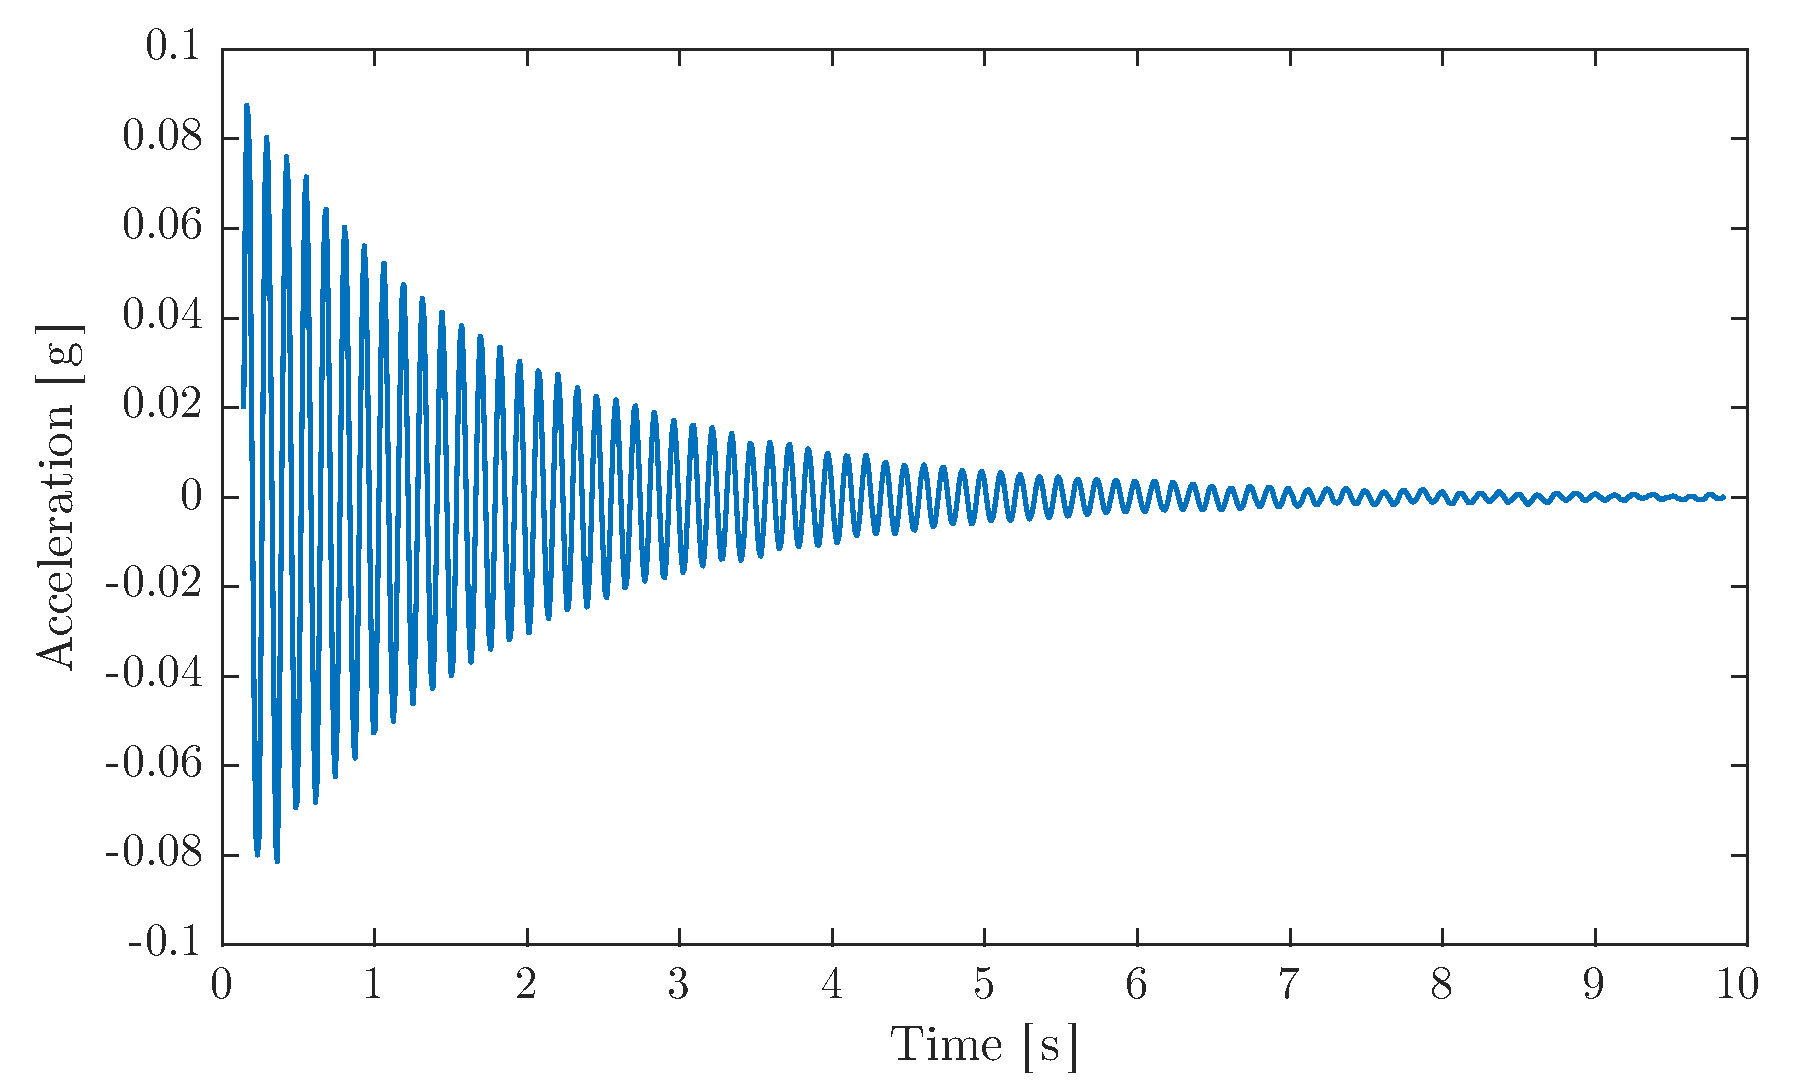
\includegraphics[width=0.8\textwidth]{resources/pdf/time_response.pdf}
		\caption{Acceleration response of the system from time $\unit{\num{0.140}}{\second}$ to $\unit{\num{9.850}}{\second}$.}
	\end{figure}
	First of all, we observe that our system performs damped harmonic oscillations. It means that $\varepsilon$, the damping ratio of the system, is strictely between $0$ and $1$. \par
	Further, to compute experimental system parameters, we have to select the 1\up{st} and the $n$\up{th} \footnote{In the matlab implementation, we have chosen $n = \num{50}$.} maxima of the dataset\footnote{We have shrunken the dataset to the time interval $\left[\num{0.140}, \, \num{9.850}\right] \, \left[\second\right]$ because extreme values were unreliable.} and interpolate around both peaks to obtain more accurate values of time and acceleration :
	\begin{align*}
		t_1 & = \unit{\num{0.1621}}{\second} & a_1 & = \unit{\num{8.793e-2}}{g} \\
		t_n & = \unit{\num{6.3645}}{\second} & a_n & = \unit{\num{0.299e-2}}{g}
	\end{align*}
	\subsection{Frequency}
	The frequency $f$ of an harmonic motion is the ratio between the number of full oscillations performed by the system during a time period and that time period length.
	\begin{alignat*}{2}
		                      &  & f_d      & = \frac{n}{t_n - t_1}                               \\
		                      &  &          & = \unit{\num{7.9001}}{\hertz}                       \\
		\Leftrightarrow \quad &  & \omega_d & = 2 \pi f_d = \unit{\num{49.6380}}{\rad\per\second}
	\end{alignat*}
	We see that the experimental frequency $\omega_d$ is a bit larger than the undamped frequency $\omega_0$, altought it should be smaller or equal given that
	\begin{align*}
		\omega_d & = \omega_0 \sqrt{1 - \varepsilon^2} \leq \omega_0
	\end{align*}
	It means that either our measures or our parameters ($m$ or $k$) are imprecise.
	\subsection{Logartihmic decrement}
	The logarithmic decrement $\Delta$ is defined by the neperian logarithm of the ratio between the amplitudes of two successive maxima. That ratio, and thus $\Delta$, is theoretically constant all along the harmonic motion. From its definition, it is easy to show that
	\begin{comment}
	\begin{align*}
		\Delta & = \ln \left(\frac{a_k}{a_{k+1}}\right)                                                                                         \\
		       & = \ln \left(\frac{1}{a_1} \frac{a_1}{a_{2}} \frac{a_2}{a_{3}} \cdots \frac{a_{k - 1}}{a_{k}} a_k \frac{a_{k}}{a_{k+1}} \right) \\
		       & = k \Delta + \ln \left(\frac{a_k}{a_1} \right)                                                                                 \\
		       & = \frac{ \ln \left(\frac{a_1}{a_k} \right) }{k - 1} \quad \forall k > 1
	\end{align*}
	\end{comment}
	\begin{equation*}
		\Delta = \ln \left(\frac{a_k}{a_{k+1}}\right) = \ldots = \frac{ \ln \left(\frac{a_1}{a_k} \right) }{k - 1} \quad \forall k > 1
	\end{equation*}
	Replacing with our computed values $a_1$ and $a_n$, we obtain
	\begin{align*}
		\Delta & = \frac{ \ln \left(\frac{a_1}{a_n} \right) }{n - 1} = \num{6.9002e-2}
	\end{align*}
	\subsection{Damping ratio}
	The value of the damping ratio $\varepsilon$ is usually computed according to its definition :
	\begin{align*}
		\varepsilon = \frac{c}{2 m \omega_0}
	\end{align*}
	In this case, the damping $c$ of the system is unknown. However, the damping ratio can still be estimated by the logarithmic decrement divided by $2 \pi$.
	\begin{align*}
		\varepsilon & \simeq \frac{\Delta}{2 \pi} = \num{1.0982e-2}
	\end{align*}
	\setcounter{section}{4}
	\section{Bode diagram}
	In the amplitude Bode diagram, we can observe a spike in amplitude near the natural frequency of the system. Searching for more accuracy, we can interpolate around the peak and obtain $X$, the maximum amplitude, and $\omega_b$, its associated frequency.
	\begin{align*}
		X & = \unit{\num{0.8116}}{g\per\newton} & \omega_b & = \unit{\num{49.7242}}{\radian\per\sec}
	\end{align*}
	\begin{figure}[h]
		\centering
		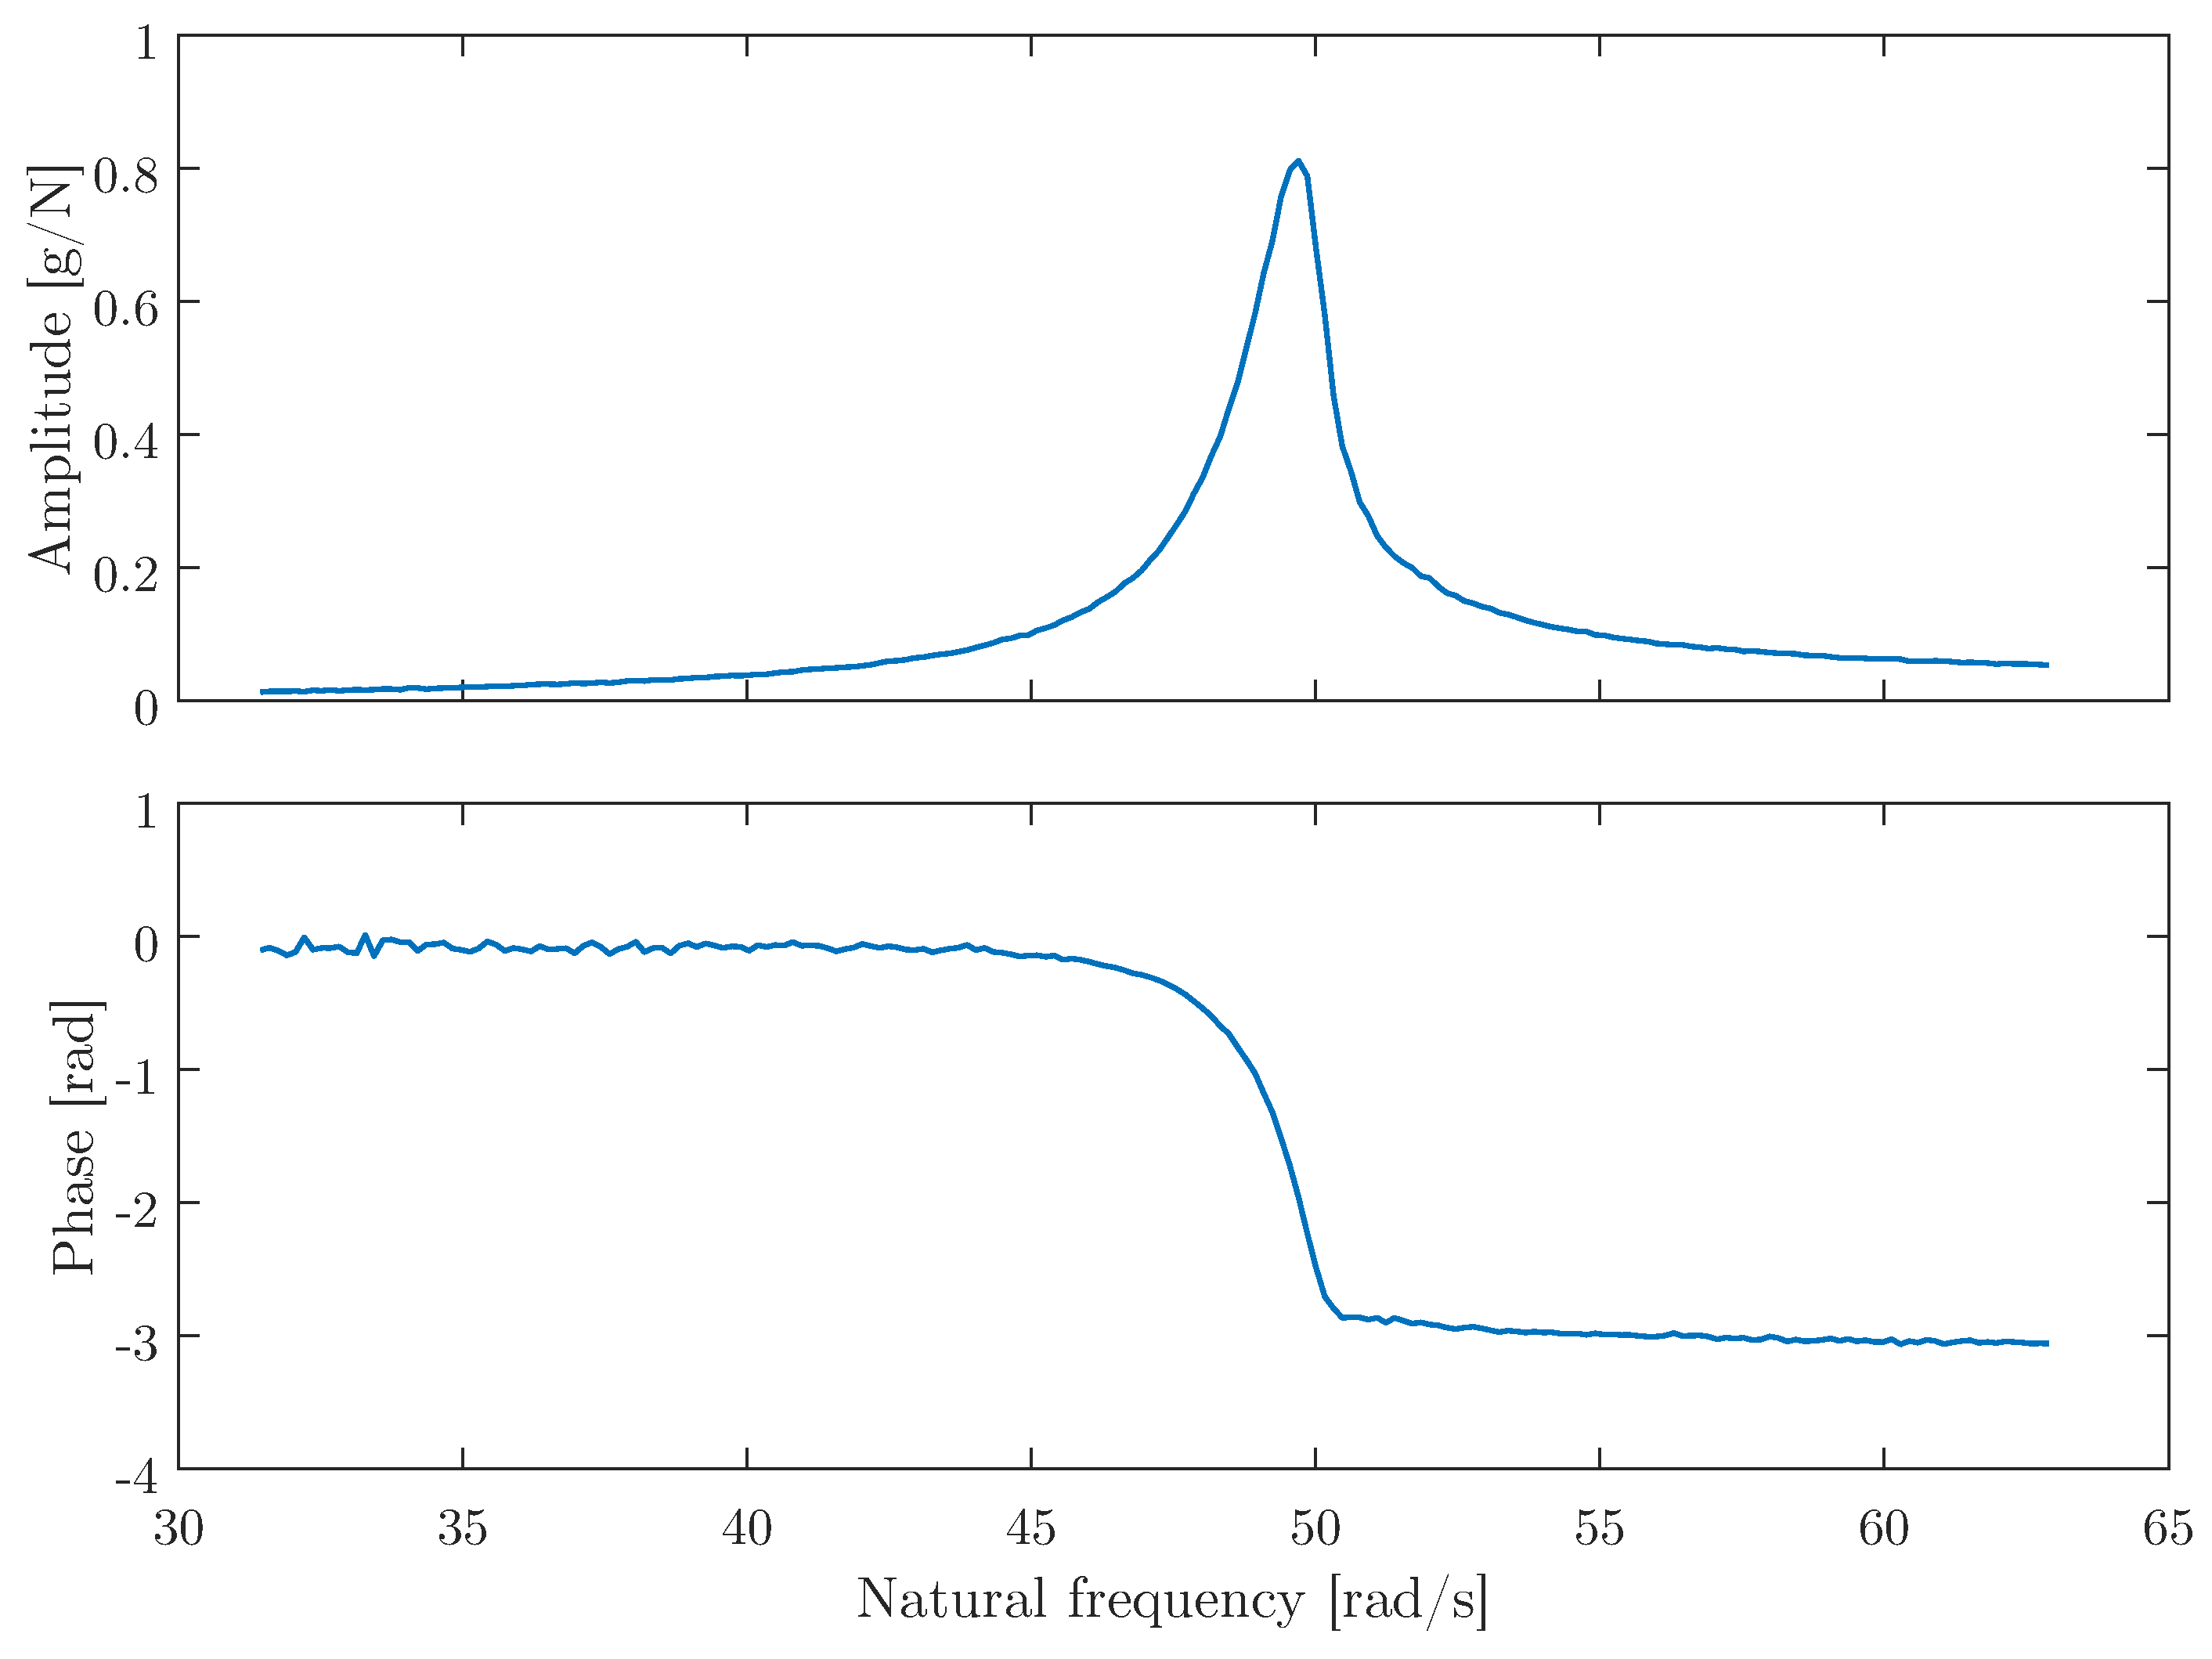
\includegraphics[width=0.8\textwidth]{resources/pdf/bode.pdf}
		\caption{Bode diagrams.}
	\end{figure}
	\subsection{Quality factor}
	The half-power method's first step is to find the frequencies $\omega_-$ and $\omega_+$ for which the amplitude is equal to $\frac{X}{\sqrt{2}}$. These can be found by interpolating separately each side of the amplitude Bode diagram's peak. In doing so, we obtain
	\begin{align*}
		\omega_- & = \unit{\num{48.9125}}{\radian\per\sec} & \omega_+ & = \unit{\num{50.1696}}{\radian\per\sec}
	\end{align*}
	We can now compute the quality factor $Q$ of the system
	\begin{align*}
		Q & = \frac{\omega_b}{\Delta \omega} = \frac{\omega_b}{\omega_+ - \omega_-} \\
		  & = \num{38.494}
	\end{align*}
	\subsection{Damping ratio}
	The damping ratio can be directly estimated from the quality factor.
	\begin{align*}
		\varepsilon & \simeq \frac{1}{2 Q} = \num{1.299e-2}
	\end{align*}
	\section{Nyquist diagram}
	\begin{figure}[h]
		\centering
		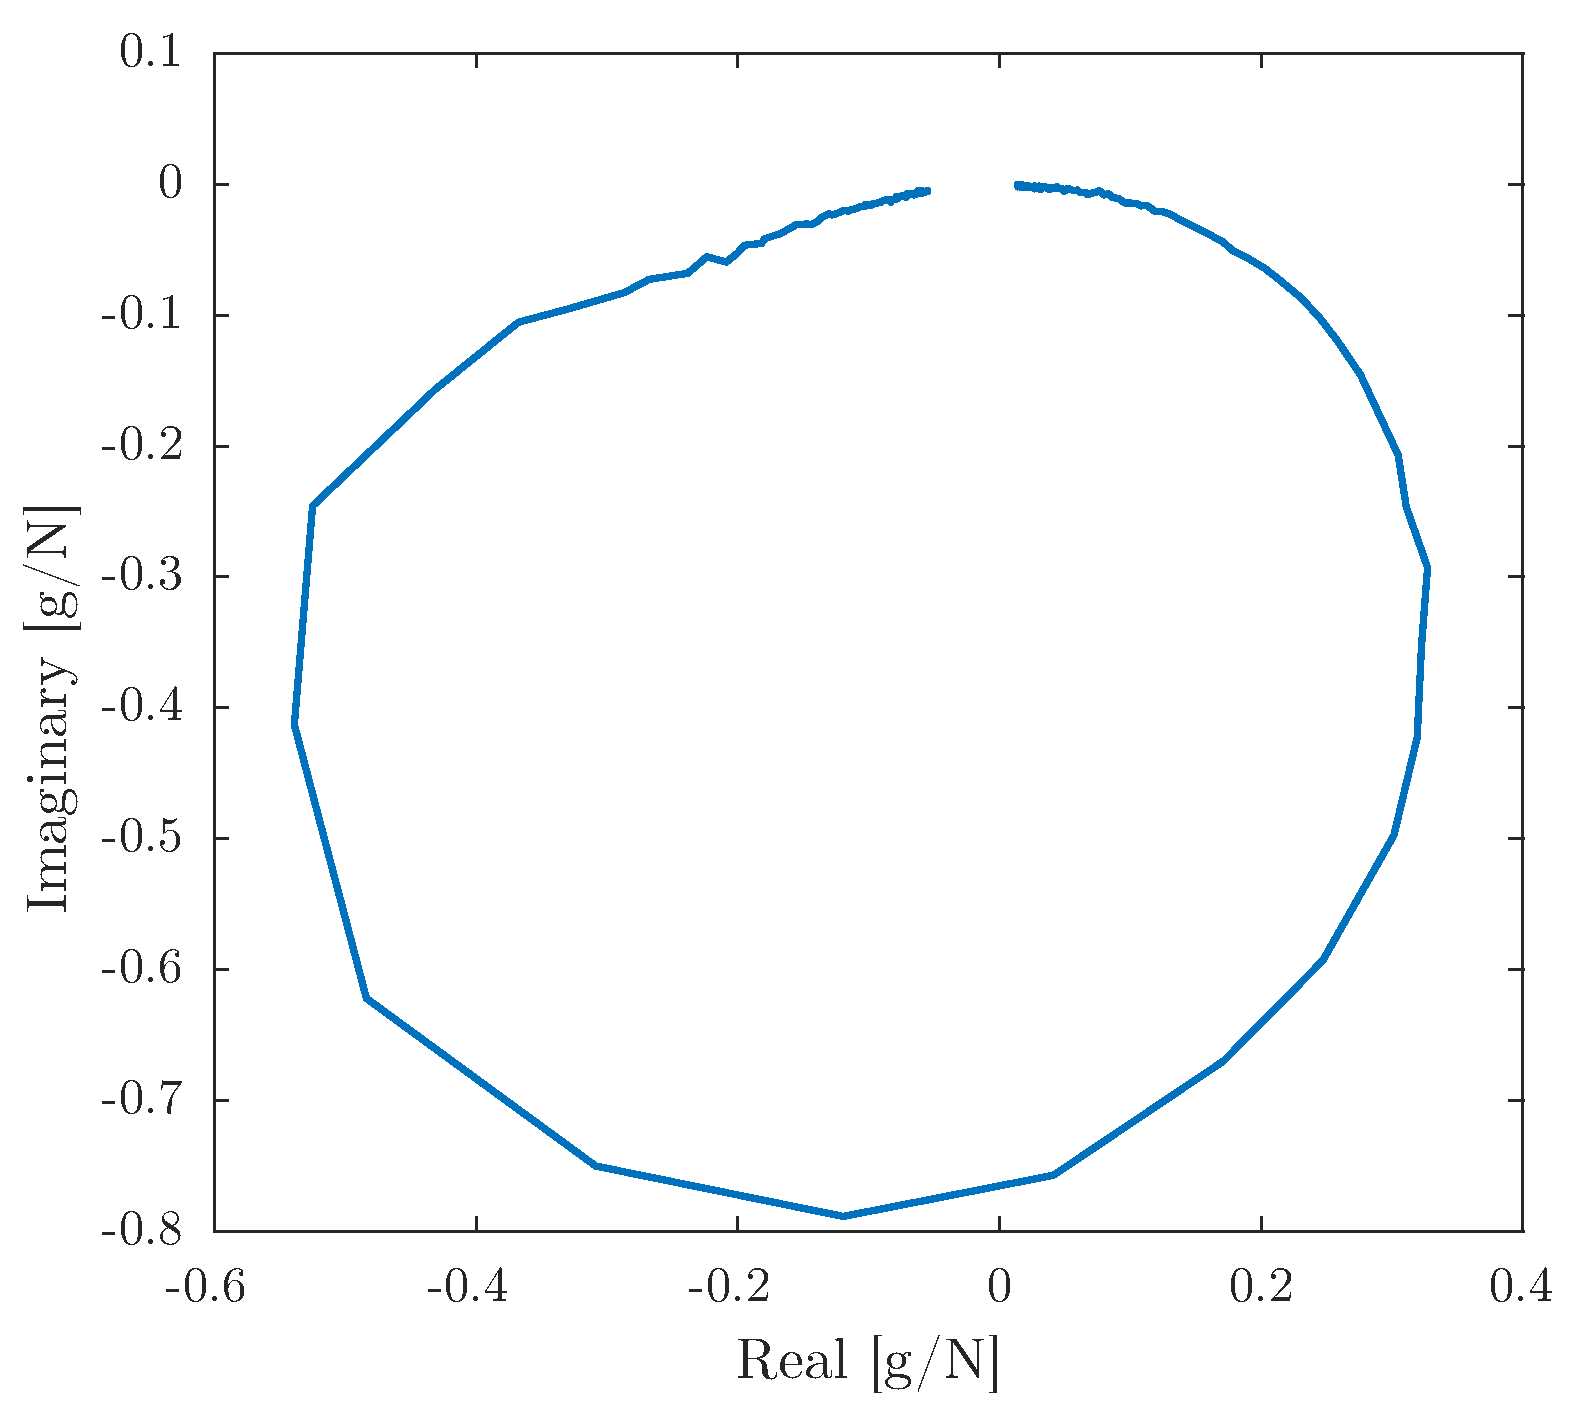
\includegraphics[width=0.5\textwidth]{resources/pdf/nyquist.pdf}
		\caption{Nyquist diagram.}
	\end{figure}
	\subsection{Quality factor}
	The quality factor can also be estimated by the amplitude\footnote{The amplitude has to be normed. In our case it means to multiply the amplitude by $m$.} at the phase resonance, described by a null real part. Firstly, we have to find the phase resonance frequency $\omega_n$ by interpolating around the real part root, which gives us
	\begin{align*}
		\omega_n = \unit{\num{49.4366}}{\radian\per\sec}
	\end{align*}
	It is now possible to determine the amplitude $X_n$ associated to $\omega_n$.
	\begin{align*}
		X_n & = \sqrt{\Re \left({\bm X}\right)^2 + \Im \left({\bm X}\right)^2} = \left|\Im \left({\bm X}\right)\right| \\
			& = \unit{\num{0.7723}}{g\per\newton} = \unit{\num{7.5759}}{m\per\second\squared\usk\newton} 
	\end{align*}
	And, therefore, the quality factor.
	\begin{align*}
		Q & \simeq m X_n = \num{33.9704}
	\end{align*}
	\subsection{Damping ratio}
	Finally, with the same estimation than before
	\begin{align*}
		\varepsilon & \simeq \frac{1}{2 Q} = \num{1.472e-2}
	\end{align*}
	\section{Conclusion}
	We can observe that either the time response, the Bode diagram or the Nyquist diagram gave us approximatively the same results :
	\begin{align*}
		\varepsilon & \approx 1 \%
	\end{align*}
	This shows that, as expected, all these methods are effective. Therefore, the choice between one or another should be lead by its convenience which varies from case to case.
\end{document}
